\begin{figure}
    \centering

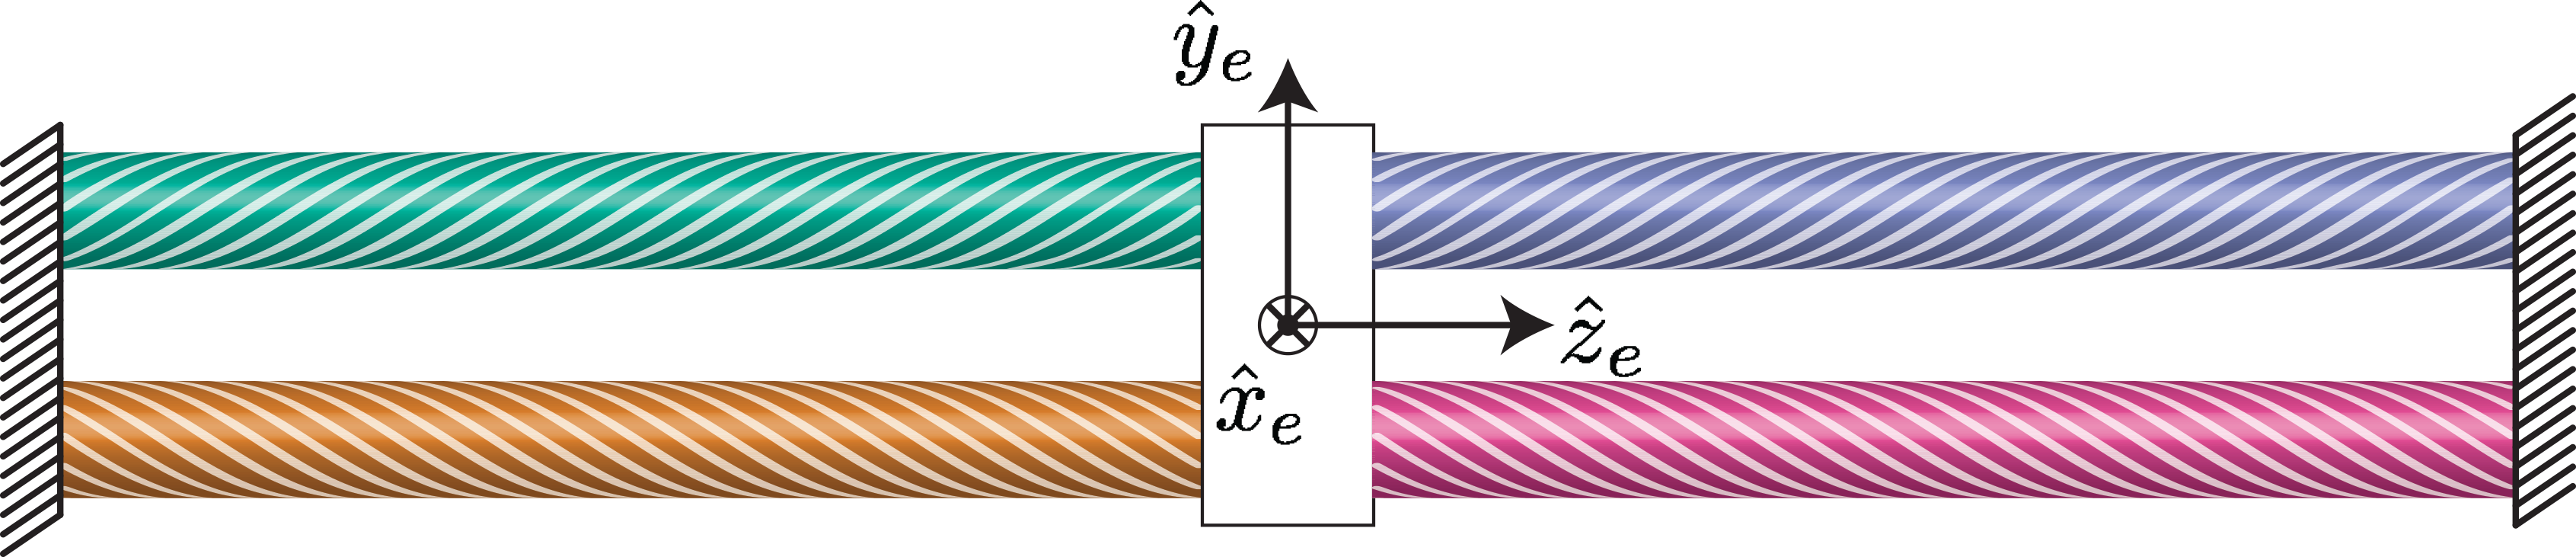
\includegraphics[width=0.85\linewidth]{figures/zntpExampleRig3.png}

\begin{tikzpicture}
\def\scl{0.45} % define scale variable for plots

% PRACTICE PLOT
\matrix [row sep=0.25cm, column sep=0cm, style={align=center}] (my matrix) at (0,0)
{

\begin{axis}[
    view={90}{0},
    axis lines=center,
    % axis equal image,
    xlabel={$M^{\hat{x}_e}$},
    ylabel={$F^{\hat{z}_e}$},
    zlabel={$M^{\hat{z}_e}$},
    ymin=-7, ymax=7, ytick={0}, %ylabel near ticks,
    xmin=-5, xmax=10, xtick={0}, %xticklabel=$\pgfmathprintnumber{\tick}^\circ$, xlabel near ticks, 
    zmin=-7, zmax=7, ztick={0}, %z dir=reverse,
    xlabel style={anchor=north}, ylabel style={anchor=north},
    scale=\scl,
    anchor=center,
    name=plot1,
    ]
    \def\pa{(-2,-3,2)}
    \def\pb{(2,-3,-2)}
    \def\pc{(2,3,-2)}
    \def\pd{(-2,3,2)}
    \addplot3[->, line width=1pt, plgreen] coordinates {(0,0,0) \pa};
%    \addplot3[->, line width=1pt, plorange] coordinates {(0,0,0) \pb};
%    \addplot3[->, line width=1pt, plpurple] coordinates {(0,0,0) \pc};
%    \addplot3[->, line width=1pt, plpink] coordinates {(0,0,0) \pd};
    % connector lines for perspective
    \addplot3[dotted] coordinates {(0,0,0) (-2,-3,0)};
    \addplot3[dotted] coordinates {(-2,-3,0) \pa}; 
%    \addplot3[dotted] coordinates {(0,0,0) (2,-3,0)};
%    \addplot3[dotted] coordinates {(2,-3,0) \pb};
%    \addplot3[dotted] coordinates {(0,0,0) (2,3,0)};
%    \addplot3[dotted] coordinates {(2,3,0) \pc};
%    \addplot3[dotted] coordinates {(0,0,0) (-2,3,0)};
%    \addplot3[dotted] coordinates {(-2,3,0) \pd};
    % faces of shape
%    \addplot3[patch, opacity=0.3, fill=black!20, faceted color=black, patch type=rectangle] 
%        coordinates {
%                    (0,0,0) \pa (0,-6,0) \pb
%                    (0,0,0) \pb (4,0,-4) \pc
%                    (0,0,0) \pc (0,6,0) \pd
%                    (0,0,0) \pd (-4,0,4) \pa
%                    };
\end{axis};

&

\begin{axis}[
    view={90}{0},
    axis lines=center,
    % axis equal image,
    xlabel={$M^{\hat{x}_e}$},
    ylabel={$F^{\hat{z}_e}$},
    zlabel={$M^{\hat{z}_e}$},
    ymin=-7, ymax=7, ytick={0}, %ylabel near ticks,
    xmin=-5, xmax=10, xtick={0}, %xticklabel=$\pgfmathprintnumber{\tick}^\circ$, xlabel near ticks, 
    zmin=-7, zmax=7, ztick={0}, %z dir=reverse,
    xlabel style={anchor=north}, ylabel style={anchor=north},
    scale=\scl,
    anchor=center,
    name=plot2,
    ]
    \def\pa{(-2,-3,2)}
    \def\pb{(2,-3,-2)}
    \def\pc{(2,3,-2)}
    \def\pd{(-2,3,2)}
    \addplot3[->, line width=1pt, plgreen] coordinates {(0,0,0) \pa};
    \addplot3[->, line width=1pt, plorange] coordinates {(0,0,0) \pb};
%    \addplot3[->, line width=1pt, plpurple] coordinates {(0,0,0) \pc};
%    \addplot3[->, line width=1pt, plpink] coordinates {(0,0,0) \pd};
    % connector lines for perspective
    \addplot3[dotted] coordinates {(0,0,0) (-2,-3,0)};
    \addplot3[dotted] coordinates {(-2,-3,0) \pa}; 
    \addplot3[dotted] coordinates {(0,0,0) (2,-3,0)};
    \addplot3[dotted] coordinates {(2,-3,0) \pb};
%    \addplot3[dotted] coordinates {(0,0,0) (2,3,0)};
%    \addplot3[dotted] coordinates {(2,3,0) \pc};
%    \addplot3[dotted] coordinates {(0,0,0) (-2,3,0)};
%    \addplot3[dotted] coordinates {(-2,3,0) \pd};
    % faces of shape
    \addplot3[patch, opacity=0.3, fill=black!20, faceted color=black, patch type=rectangle] 
        coordinates {
                    (0,0,0) \pa (0,-6,0) \pb
%                    (0,0,0) \pb (4,0,-4) \pc
%                    (0,0,0) \pc (0,6,0) \pd
%                    (0,0,0) \pd (-4,0,4) \pa
                    };
\end{axis};


\\

\begin{axis}[
    view={90}{0},
    axis lines=center,
    % axis equal image,
    xlabel={$M^{\hat{x}_e}$},
    ylabel={$F^{\hat{z}_e}$},
    zlabel={$M^{\hat{z}_e}$},
    ymin=-7, ymax=7, ytick={0}, %ylabel near ticks,
    xmin=-5, xmax=10, xtick={0}, %xticklabel=$\pgfmathprintnumber{\tick}^\circ$, xlabel near ticks, 
    zmin=-7, zmax=7, ztick={0}, %z dir=reverse,
    xlabel style={anchor=north}, ylabel style={anchor=north},
    scale=\scl,
    anchor=center,
    name=plot3,
    ]
    \def\pa{(-2,-3,2)}
    \def\pb{(2,-3,-2)}
    \def\pc{(2,3,-2)}
    \def\pd{(-2,3,2)}
    \addplot3[->, line width=1pt, plgreen] coordinates {(0,0,0) \pa};
    \addplot3[->, line width=1pt, plorange] coordinates {(0,0,0) \pb};
    \addplot3[->, line width=1pt, plpurple] coordinates {(0,0,0) \pc};
%    \addplot3[->, line width=1pt, plpink] coordinates {(0,0,0) \pd};
    % connector lines for perspective
    \addplot3[dotted] coordinates {(0,0,0) (-2,-3,0)};
    \addplot3[dotted] coordinates {(-2,-3,0) \pa}; 
    \addplot3[dotted] coordinates {(0,0,0) (2,-3,0)};
    \addplot3[dotted] coordinates {(2,-3,0) \pb};
    \addplot3[dotted] coordinates {(0,0,0) (2,3,0)};
    \addplot3[dotted] coordinates {(2,3,0) \pc};
%    \addplot3[dotted] coordinates {(0,0,0) (-2,3,0)};
%    \addplot3[dotted] coordinates {(-2,3,0) \pd};
    % faces of shape
    \addplot3[patch, opacity=0.3, fill=black!20, faceted color=black, patch type=rectangle] 
        coordinates {
                    (0,0,0) \pa (0,-6,0) \pb
                    (0,0,0) \pb (4,0,-4) \pc
%                    (0,0,0) \pc (0,6,0) \pd
%                    (0,0,0) \pd (-4,0,4) \pa
                    };
\end{axis};

&

\begin{axis}[
    view={90}{0},
    axis lines=center,
    % axis equal image,
    xlabel={$M^{\hat{x}_e}$},
    ylabel={$F^{\hat{z}_e}$},
    zlabel={$M^{\hat{z}_e}$},
    ymin=-7, ymax=7, ytick={0}, %ylabel near ticks,
    xmin=-5, xmax=10, xtick={0}, %xticklabel=$\pgfmathprintnumber{\tick}^\circ$, xlabel near ticks, 
    zmin=-7, zmax=7, ztick={0}, %z dir=reverse,
    xlabel style={anchor=north}, ylabel style={anchor=north},
    scale=\scl,
    anchor=center,
    name=plot4,
    ]
    \def\pa{(-2,-3,2)}
    \def\pb{(2,-3,-2)}
    \def\pc{(2,3,-2)}
    \def\pd{(-2,3,2)}
    \addplot3[->, line width=1pt, plgreen] coordinates {(0,0,0) \pa};
    \addplot3[->, line width=1pt, plorange] coordinates {(0,0,0) \pb};
    \addplot3[->, line width=1pt, plpurple] coordinates {(0,0,0) \pc};
    \addplot3[->, line width=1pt, plpink] coordinates {(0,0,0) \pd};
    % connector lines for perspective
    \addplot3[dotted] coordinates {(0,0,0) (-2,-3,0)};
    \addplot3[dotted] coordinates {(-2,-3,0) \pa}; 
    \addplot3[dotted] coordinates {(0,0,0) (2,-3,0)};
    \addplot3[dotted] coordinates {(2,-3,0) \pb};
    \addplot3[dotted] coordinates {(0,0,0) (2,3,0)};
    \addplot3[dotted] coordinates {(2,3,0) \pc};
    \addplot3[dotted] coordinates {(0,0,0) (-2,3,0)};
    \addplot3[dotted] coordinates {(-2,3,0) \pd};
    % faces of shape
    \addplot3[patch, opacity=0.3, fill=black!20, faceted color=black, patch type=rectangle] 
        coordinates {
                    (0,0,0) \pa (0,-6,0) \pb
                    (0,0,0) \pb (4,0,-4) \pc
                    (0,0,0) \pc (0,6,0) \pd
                    (0,0,0) \pd (-4,0,4) \pa
                    };
\end{axis};

\\
};

\node[above] (a2) at ($ (plot1.south west) !0.1! (plot1.south east) $) {(a)};
\node[above] (b2) at ($ (plot2.south west) !0.1! (plot2.south east) $) {(b)};
\node[above] (c2) at ($ (plot3.south west) !0.1! (plot3.south east) $) {(c)};
\node[above] (d2) at ($ (plot4.south west) !0.1! (plot4.south east) $) {(d)};

\end{tikzpicture}

    \caption{An end effector is driven by the parallel combination of two pairs of FREEs with opposing chirality.
    The zonotope (grey areas) is the range of forces that can be produced by applying strictly positive pressure to the individual FREEs.
    It is spanned by the individual force vectors that each FREE produces at maximal pressure (plotted here in the color corresponding to the FREE's appearance in the diagram above).
    By constructing the zonotope for (a) one FREE, (b) two FREEs, (c) three FREEs, (d) four FREEs in parallel, one can observe that all four actuators are needed to gain full control authority over forces along and torques about the $z$-axis.
    In this poorly designed system (with fiber angles and attachments points as shown in the top diagram), the theoretical minimum of 3 actuators is not sufficient to achieve full control authority.}
    \label{fig:zntpConstructed}
\end{figure}